% TEMPLATE for Usenix papers, specifically to meet requirements of
%  USENIX '05
% originally a template for producing IEEE-format articles using LaTeX.
%   written by Matthew Ward, CS Department, Worcester Polytechnic Institute.
% adapted by David Beazley for his excellent SWIG paper in Proceedings,
%   Tcl 96
% turned into a smartass generic template by De Clarke, with thanks to
%   both the above pioneers
% use at your own risk.  Complaints to /dev/null.
% make it two column with no page numbering, default is 10 point

% Munged by Fred Douglis <douglis@research.att.com> 10/97 to separate
% the .sty file from the LaTeX source template, so that people can
% more easily include the .sty file into an existing document.  Also
% changed to more closely follow the style guidelines as represented
% by the Word sample file. 

% Note that since 2010, USENIX does not require endnotes. If you want
% foot of page notes, don't include the endnotes package in the 
% usepackage command, below.

% This version uses the latex2e styles, not the very ancient 2.09 stuff.
% \documentclass[letterpaper,twocolumn,10pt]{article}
\pdfminorversion=4

\documentclass{hotnets15}

\usepackage{epsfig,endnotes}
\usepackage{color}
\usepackage{colortbl}
\usepackage{verbatim}
\usepackage[font=bf]{caption}
\usepackage{xspace}
\usepackage{mdframed}
\usepackage{float}
\usepackage{microtype}
\usepackage{newtxmath}

\usepackage{tikz}
\usepackage{enumitem}
\usepackage{booktabs}  % for toprule, bottomrule in tables
\usepackage[sort,space]{cite}
\usepackage{flushend}  % for balanced final columns


\usepackage{graphicx}
\usepackage{caption}
\usepackage{subfigure}

\newcommand{\subparagraph}{}
\usepackage[compact]{titlesec}

\usepackage{url}


\newcommand{\tightcaption}[1]{\vspace{-0.3cm}\caption{#1}\vspace{-0.3cm}}
\newcommand{\tightsection}[1]{\section{#1}}
\newcommand{\tightsubsection}[1]{\subsection{#1}}
\newcommand{\tightsubsubsection}[1]{\subsubsection{#1}}

\newcommand{\eg}{{\it e.g.,}\xspace}
\newcommand{\ie}{{\it i.e.,}\xspace}

\newcounter{note}[section]
\renewcommand{\thenote}{\thesection.\arabic{note}}

\newcommand{\Section}{\S}

\usepackage{pifont}
\newcommand{\cmark}{\ding{51}}%
\newcommand{\xmark}{\ding{55}}%

\newcommand{\fillme}{{\bf XXX}~}

\definecolor{purple}{RGB}{175,0,255}


\newcommand{\mypara}[1]{\medskip\noindent{\bf {#1}:}~}
\newcommand{\myparatight}[1]{\smallskip\noindent{\bf {#1}:}~}
\newcommand{\myparaq}[1]{\smallskip\noindent{\bf {#1}?}~}
\newcommand{\mysubparatight}[1]{\noindent {\it {#1}:}~}

%-- place any standard commands/environments here to get included in
%-- documents.  When you include this file, you should do it before
%-- the \begin{document} tag.

%%%%%%%%%%%%%%%%%%%%%%%%%%%%%%%%%%%%%%%%%%%%%%%%%%%%%%%%%%%%%%%%%%%%%%
%-- CHANGES:
%-- 07/31/01 -jstrunk- Added command to set the paper margins.

%-- Provides fixed width font for commands and code snips.
\newcommand{\code}[1]{\texttt{\textbf{#1}}}

%-- Terms...  Use this to introduce a term in the paper.
\newcommand{\term}[1]{\emph{#1}}

%-- Provides stylization for e-mail addresses
%\newcommand{\email}[1]{\emph{(#1)}}

%-- Starts a minor section (puts the title inline w/ the text.
\newcommand{\minorsection}[1]{\textbf{#1}:}

%-- Jiri caption
\newcommand{\minicaption}[2]{\caption[#1]{\textbf{#1.} #2}}

%-- Units on numbers: 4KB -> \units{4}{KB}
\newcommand{\units}[2]{#1~#2}

%-- Commands...  i.e. WRITE commands.
\newcommand{\command}[1]{{\sc \MakeLowercase{#1}}}

%-- For notes about things that need to be fixed.
\newcommand{\fix}[1]{\marginpar{\LARGE\ensuremath{\bullet}}
    \MakeUppercase{\textbf{[#1]}}}
%-- For adding inline notes to a draft preceded by your initials
%-- E.g., \fixnote{JJW}{What the heck is a foobar?}
\newcommand{\fixnote}[2]{\marginpar{\LARGE\ensuremath{\bullet}}
    {\textbf{[#1:} \textit{#2\,}\textbf{]}}}

%-- Setting margins: \setmargins{left}{right}{top}{bottom}
\newcommand{\setmargins}[4]{
    % Calculations of top & bottom margins
    \setlength\topmargin{#3}
    \addtolength\topmargin{-.5in}  %-- seems like this should be 1, but .5
                                   %-- balances the text top to bottom
    \addtolength\topmargin{-\headheight}
    \addtolength\topmargin{-\headsep}
    \setlength\textheight{\paperheight}
    \addtolength\textheight{-#3}
    \addtolength\textheight{-#4}

    % Calculations of left & right margins
    \setlength\oddsidemargin{#1}
    \addtolength\oddsidemargin{-1in}
    \setlength\evensidemargin{\oddsidemargin}
    \setlength\textwidth{\paperwidth}
    \addtolength\textwidth{-#1}
    \addtolength\textwidth{-#2}
}

%-- For the tabularx environment... Using L, C, R as the column type
%-- will left, center, or right justify the text.
\newcolumntype{L}{X}
\newcolumntype{C}{>{\centering\arraybackslash}X}
\newcolumntype{R}{>{\raggedleft\arraybackslash}X}

%-- To comment out a swatch of text, use \omitit{blah blah blah}
\long\def\omitit#1{}

%-- Inline title; useful for sub-sub-sections in which you don't want a separate
%-- line for the title.
\newcommand{\inlinesection}[1]{\smallskip\noindent{\textbf{#1.}}}


%%%
%%% COMMENTS / TODOS
%%%
\usepackage{ifthen}
\usepackage{xcolor}
\newcommand{\exclude}[1]{}
\newcommand{\showComments}{yes}
\newcommand{\note}[2]{
    \ifthenelse{\equal{\showComments}{yes}}{\textcolor{#1}{#2}}{}
}
\newcommand{\TODO}[1]{%
	\addcontentsline{tdo}{todo}{\protect{#1}}%
	\note{red}{TODO: #1}
}

\makeatletter \newcommand{\listoftodos}
{\section*{Todo List} \@starttoc{tdo}}
\newcommand{\l@todo}
{\@dottedtocline{1}{0em}{2.3em}} \makeatother


\newcommand{\myparaittight}[1]{\smallskip\noindent{\emph {#1}:}~}
\newcommand{\question}[1]{\smallskip\noindent{\emph{Q:~#1}}\smallskip}
\newcommand{\myparaqtight}[1]{\smallskip\noindent{\bf {#1}}~}
\newcommand{\jc}[1]{\note{green}{[HZ: #1]}}
\newcommand{\matt}[1]{\note{blue}{[MKM: #1]}}
\newcommand{\srini}[1]{\note{magenta}{[SS: #1]}}
\newcommand{\bruce}[1]{\note{red}{[BMM: #1]}}
\newcommand{\nadi}[1]{\note{purple}{[INB: #1]}}
\newcommand{\mycomment}[1]{}

\newcounter{packednmbr}

\newenvironment{packedenumerate}{\begin{list}{\thepackednmbr.}{\usecounter{packednmbr}\setlength{\itemsep}{0.5pt}\addtolength{\labelwidth}{-4pt}\setlength{\leftmargin}{\labelwidth}\setlength{\listparindent}{\parindent}\setlength{\parsep}{1pt}\setlength{\topsep}{0pt}}}{\end{list}}

\newenvironment{packeditemize}{\begin{list}{$\bullet$}{\setlength{\itemsep}{0.5pt}\addtolength{\labelwidth}{-4pt}\setlength{\leftmargin}{\labelwidth}\setlength{\listparindent}{\parindent}\setlength{\parsep}{1pt}\setlength{\topsep}{0pt}}}{\end{list}}


%
\def\sharedaffiliation{%
\end{tabular}
\begin{tabular}{c}}
%

\begin{document}

\title{Characterizing Reconfigurable Topologies in Datacenter Fabrics}

\numberofauthors{1}
\author{\alignauthor Paper \#16, 7 pages}


\maketitle



\subsection*{Abstract} 

\section{Introduction}
\label{sec:intro}

%% Maybe use some of this from SOLSTICE?
%% Today's datacenters aggregate tremendous amounts of compute and storage
%% capacity, driving demand for network switches with ever-increasing port counts
%% and line speeds.  However, supporting these demands with existing packet
%% switching technology is becoming increasingly expensive---in cost, heat, power,
%% and cabling. Packet switches are flexible, capable of making forwarding
%% decisions at the granularity of individual packets.  In common modern scenarios,
%% however, this flexibility is unnecessary: many (often consecutive) packets are
%% sent to the same output port.  Two key factors contribute to this traffic
%% pattern. First, traffic inside a datacenter often has high spatial locality,
%% where a large fraction of the traffic that enters each switch port is destined
%% for only a small number of output ports~\cite{msft-imc09, facebook:sigcomm15}.
%% Second, traffic is often bursty, with significant temporal locality between
%% packets sharing the same destination~\cite{bullet:conext13,
%%   facebook:sigcomm15}. The consequence of these two factors is that the traffic
%% demand matrix at a datacenter switch is often both skewed and
%% sparse~\cite{mordia:hotnets12,flyways,augmenting-dc-wireless}.

%% \begin{figure*}[t!!!]
%% \centering
%% 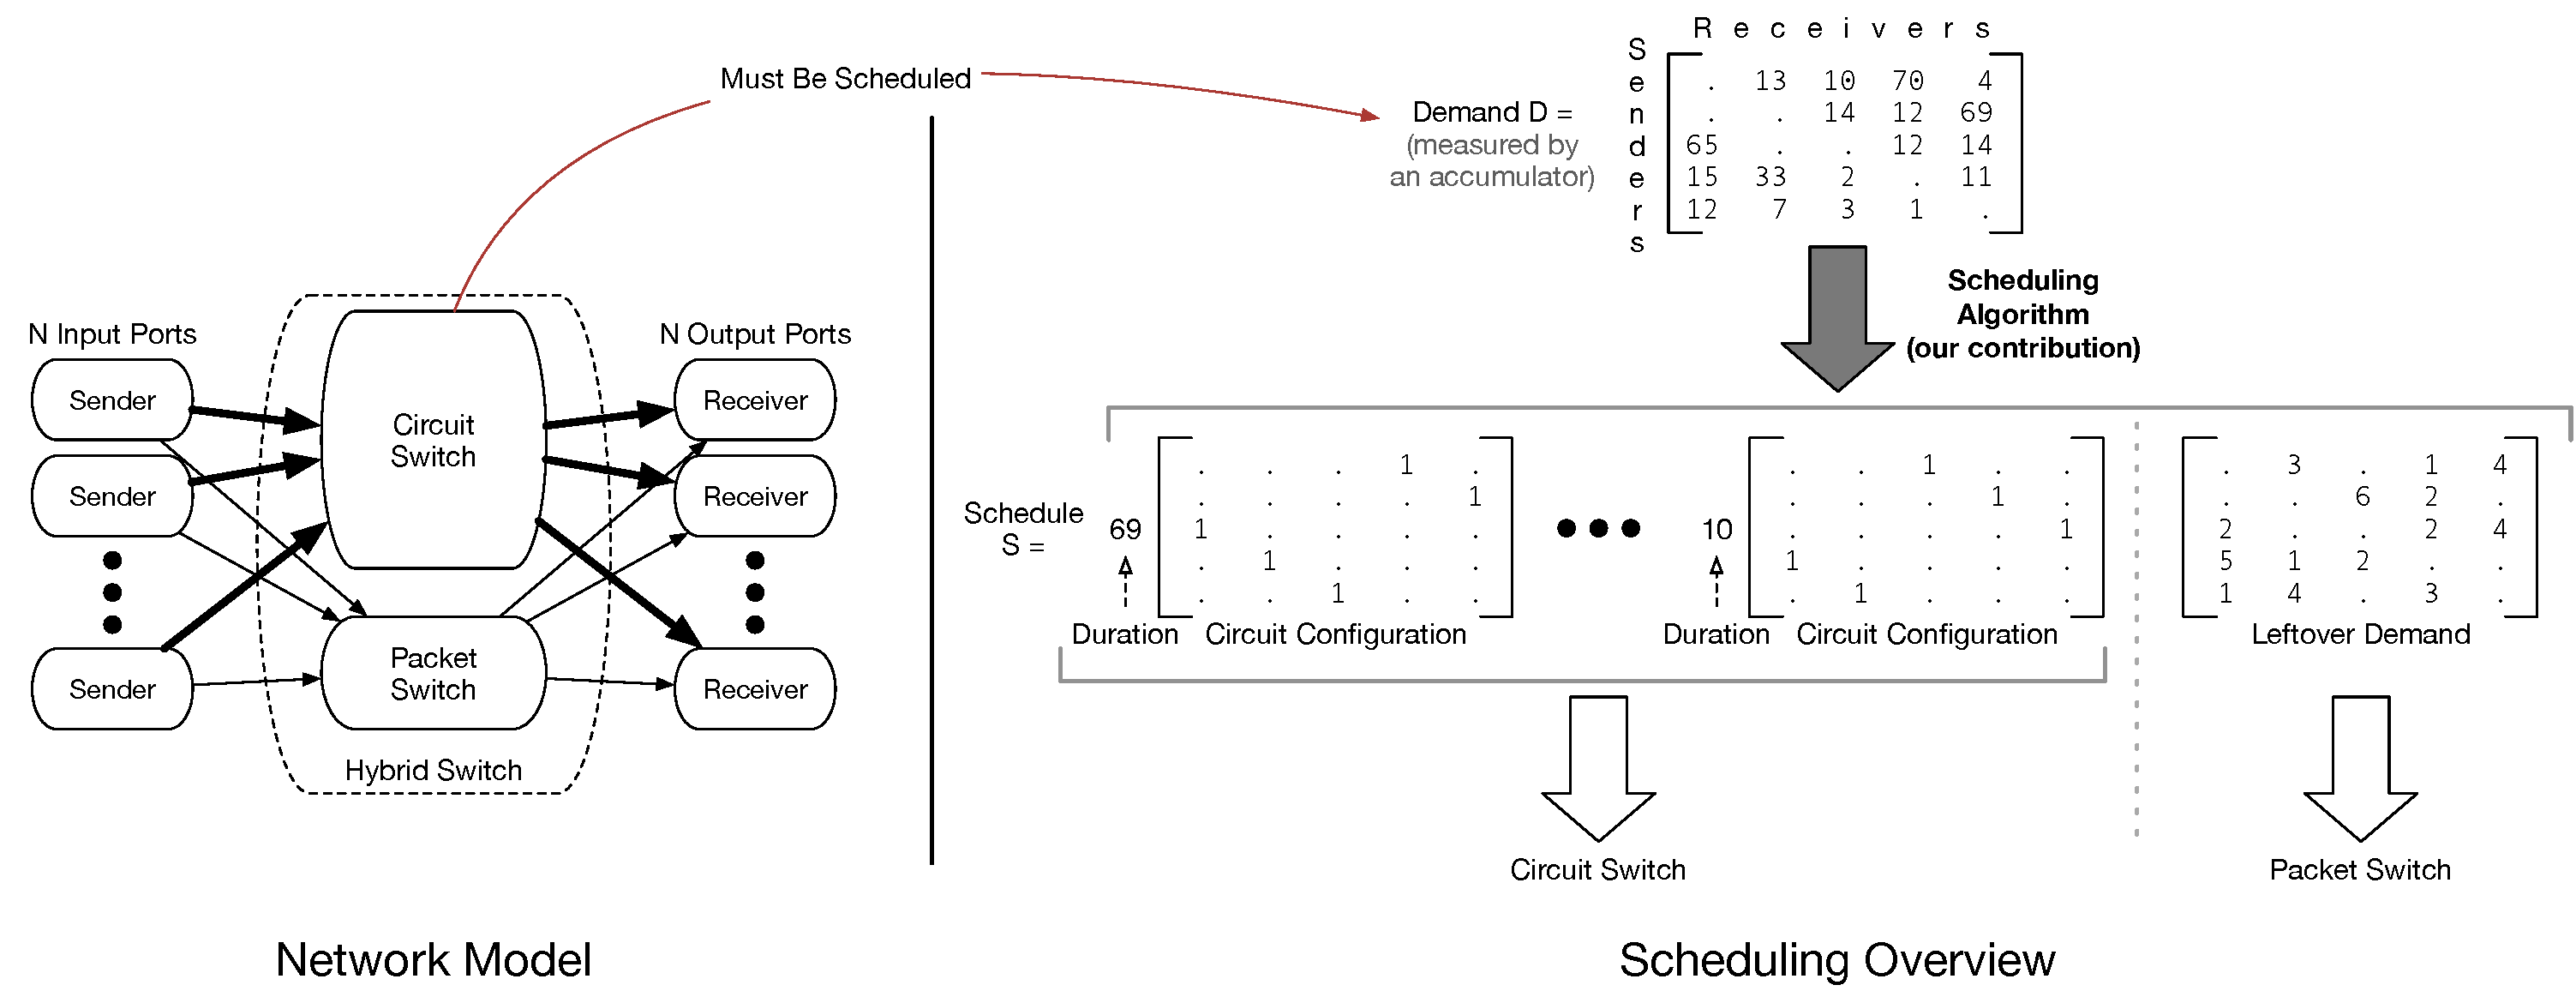
\includegraphics[width=1\textwidth]{figures/setting}
%% \caption{Our model of a hybrid switch architecture and the scheduling
%%   process. The circuit switch has high bandwidth, but slow reconfiguration
%%   time. The packet switch has low bandwidth (e.g., an order of magnitude lower),
%%   but can make forwarding decisions per-packet.
%%   %Both switches must have high utilization.
%%   }
%% \label{fig:arch}
%% \end{figure*}

%% Researchers have seized upon these observations to propose hybrid datacenter
%% network architectures that offer higher throughput at lower cost by combining
%% high-speed optical~\cite{OSA,helios:sigcomm10,c-Through} or
%% wireless~\cite{flyways,augmenting-dc-wireless,mirror-mirror} circuit switching
%% technologies with traditional electronic packet switches. Typically, the circuit
%% switch has a significantly higher data rate than the packet switch, but incurs a
%% non-trivial reconfiguration penalty. While the potential cost savings that
%% hybrid techniques could realize is large, the design space of scheduling
%% algorithms that enable high utilization in hybrid networks is not yet well
%% understood. Earlier work that considers circuit switches with substantial
%% reconfiguration delay offers no guidance about how to negotiate the trade-off
%% between remaining in the current (potentially sub-optimal) circuit configuration
%% vs. incurring a costly reconfiguration delay to switch to a potentially better
%% circuit configuration~\cite{c-Through, helios:sigcomm10, wang:hotnets}.  The
%% reconfiguration cost of these systems was so high that they were forced to keep
%% a configuration pinned up for a relatively long period anyway.

%% In recent years, however, the switching time of optical circuit switches has
%% improved substantially~\cite{mordia:sigcomm13}. As a result, an efficient
%% scheduling algorithm for a modern hybrid design must determine: 1) a set of
%% circuit configurations (which ports are connected to which other ports and how
%% long that configuration should remain in effect) designed to maximize the
%% traffic serviced over the high-bandwidth but slow-to-reconfigure
%% circuit-switched network, and 2) what traffic should be sent to the
%% low-bandwidth but flexible packet switch.

%% Computing an optimal set of circuit configurations to maximize circuit-switched
%% utilization has no known polynomial-time algorithms, scaling as $O(n!)$ in the
%% number of switch ports (\S\ref{sec:optimization}). The challenge arises due to
%% the non-trivial switching time between configurations, which necessitates not
%% only sending as much traffic as possible, but doing so in the fewest number of
%% configurations.

%% The end goal of this paper is an effective and fast heuristic algorithm that
%% delivers high switch utilization. To this end, we first provide a detailed
%% characterization of the problem plus an optimal (but impractical) solution that
%% sheds light on how to design an effective heuristic.  We then present our
%% heuristic, Solstice, which provides 2.9$\times$ higher utilization compared to
%% previous algorithms by taking advantage of the known sparsity and skew of
%% datacenter workloads---some of the same features that make the traditional
%% scheduling problem hard.

%% The contributions of this work are as follows:
%% \begin{enumerate}
%% \item Characterizing the hybrid switch scheduling problem.
%% \item Exploring the design space of hybrid scheduling:
%%   \begin{packedenumerate}
%%     \item \myparatight{Lower bound} an instantly computable but loose bound on
%%       the minimum amount of time it takes to serve all demand (but provides no
%%       actual schedules).
%%     \item \myparatight{Optimal scheduling} optimally schedule all
%%       demand with minimal time; impossible to run in real time at scale.
%%     \item \myparatight{Heuristic algorithm (``Solstice'')} runs in real time at
%%       scale, but slightly underperforms optimal (by at most 14\%
%%       at target scale).
%%     \item \myparatight{Heuristic + optimization (``\mbox{Solstice{}++}'')} runs at
%%       scale (though not in real time), but tightens the gap between Solstice and
%%       optimal (at most 12\% from optimal at target scale).
%%   \end{packedenumerate}
%% \item Insight into the challenges and benefits of using hybrid switches, with a
%%   focus on high circuit utilization.
%% \end{enumerate}

\tightsection{The Setting}
\label{sec:setting}

\section{Problems of CDN Commoditization}
\label{sec:problems}

\section{Designing a Better Interface}
\label{sec:design}

\tightsection{Related work}
\label{sec:related}


\tightsection{Conclusion}
\label{sec:concl}



\bibliographystyle{acm}
\bibliography{ref}

\end{document}
